\section{Client �ndern}In diesem Dialog k�nnen Sie die Einstellungen eines Clients �ndern. Neben den Eingabefeldern, die Sie  bereits vom Client-Hinzuf�gen-Dialog kennen, gibt es drei Spalten, mit denen Sie bestimmen k�nnen, was mit den eingegebenen Werten geschehen soll.\\
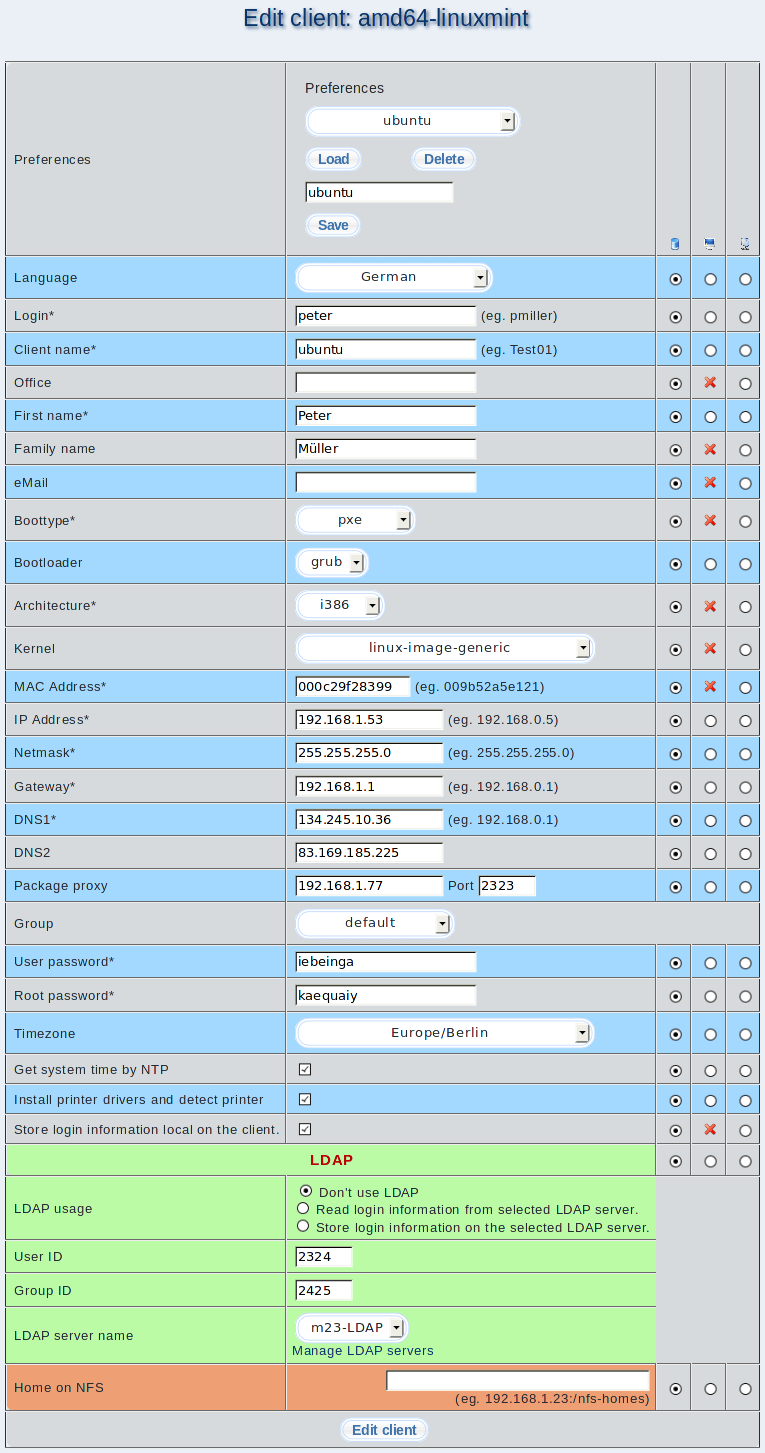
\includegraphics[scale=0.4]{/mdk/doc/manual/screenshots/de/edit_client.png} \\
\begin{itemize}
\item \textbf{Linke Spalte}: W�hlen Sie diese Spalte aus, so bleibt der im Client und auf dem Server gespeicherte Wert unangetastet.\\
\item \textbf{Mittlere Spalte}: Die �nderungen sollen auf dem Client vorgenommen und nachtr�glich mit dem Server abgeglichen werden.\\
\item \textbf{Rechte Spalte}: Es werden nur die Datenbankeintr�ge auf dem Server ge�ndert. Dies ist z.B. n�tzlich, wenn die �nderungen auf dem Client bereits per Hand vorgenommen wurden.\\
\end{itemize}
\subsection{Hinweis}
Einige Einstellungen werden nur auf dem Server vermerkt. Daher ist das �ndern auf dem Client nicht m�glich. Bei diesen kann die mittlere Spalte nicht gew�hlt werden.\\
